\section{Considera el siguiente P.P.L}


    \begin{tabular}{|l|l|}
    \hline
        Max & $-x_1+2x_2$ \\ \hline
        ~ & $2x_1+3x_2\leq 6$ \\ \hline
        ~ & $x_1-2x_2\geq -2$\\ \hline
        ~ & $x_1,x_2\geq0$ \\ \hline
    \end{tabular}
    \begin{itemize}
        \item Construya el problema dual 
        
        Tengamos que el problema primal como:

    \begin{tabular}{|l|l|}
    \hline
        $Max$ & $z=-x_1+2x_2$ \\ \hline
         & $2x_1+3x_2\leq 6: w_1$ \\ \hline
         & $x_1-2x_2\geq -2: w_3$ \\ \hline
         & $x_1,x_2\geq0$ \\ \hline
    \end{tabular} 
    Y el problema dual como:
    \begin{tabular}{|l|l|}
    \hline
        $Min$ & $z'=6w_1-2w_2$ \\ \hline
         & $2w_1+w_2\geq -1$ \\ \hline
         & $3w_1-2w_2\leq 3$ \\ \hline
         & $x_1,x_2\geq0 $\\ \hline
    \end{tabular}    
        
    
        
        
        \item Resuelva gr\'aficamente el problema dual
        
        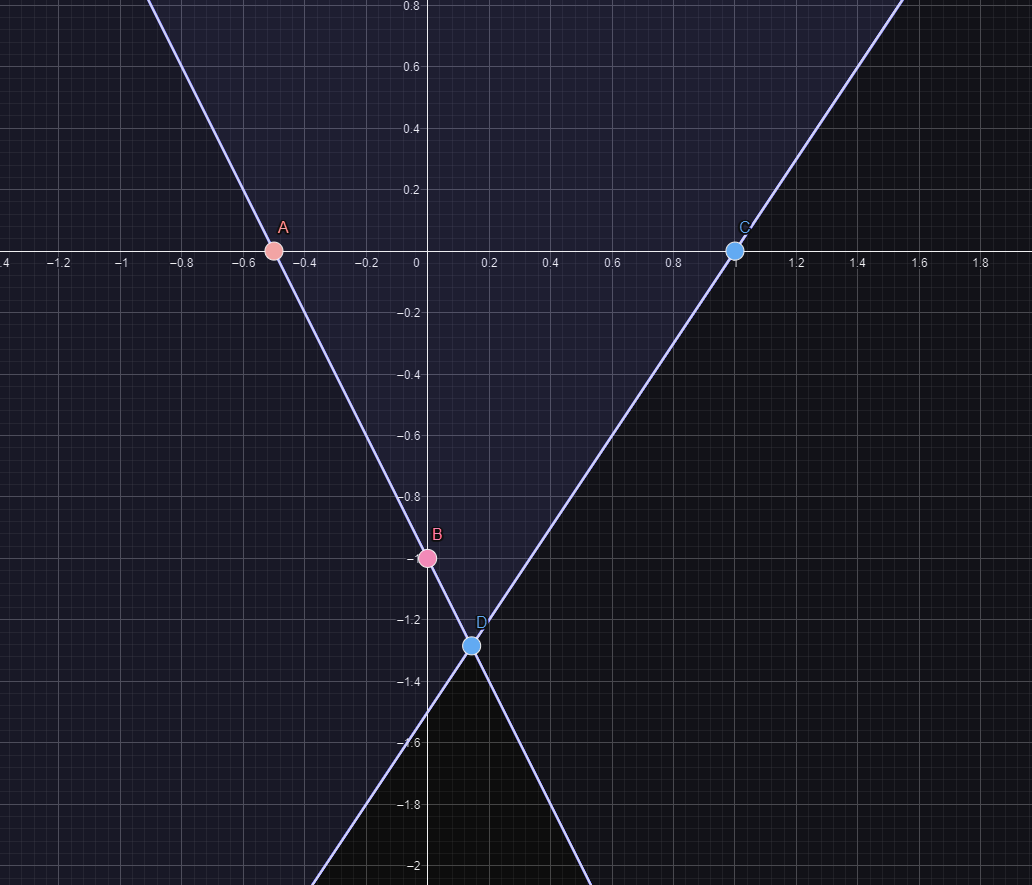
\includegraphics[scale=0.2]{Ejercicios/Imagenes/Ejercicio2a_2.png}
        
        donde:\\
        
            $A=(-0.5,0)$\\
            
            $B=(0,-\frac{3}{2})$\\
            
            $C=(1,0)$\\
            
            $D=(\frac{1}{7},-\frac{9}{7})$\\

            donde tenemos:
            $$6\left(\frac{1}{7}\right)-2\left(-\frac{9}{7}\right)=\frac{24}{7}$$
                       
            el cual es la soluci\'on
            
        \item Utilize la informaci\'on del problema dual y los teoremas de dualidad para resolver el problema primal
    
    
    \end{itemize}